\DiaryEntry{Pythagorean Triples (cont'd)}{2023-04-11}{Number Theory}

The following Figure shows the distribution of primitive Pythagorean triples for values $x, y < 2500$.

\begin{figure}[H]
    \centering
    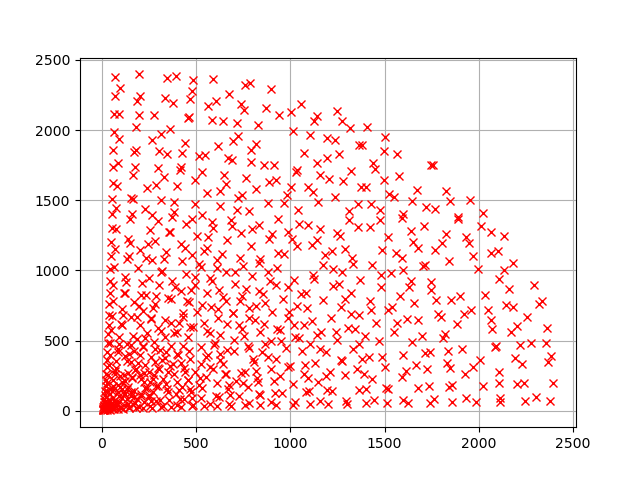
\includegraphics[scale=0.75]{images/2023-03-28-triples_2.png}
\end{figure}

There is no visible structure \todo{this is entirely true; see \href{https://en.m.wikipedia.org/wiki/Pythagorean_triple}{here} for some structure-related information}; the points seem to be randomly distributed. In total, we have $395$ points out of a total $2500^2$ points; that corresponds to a density of $\approx 6.3 \cdot 10^{-5}$. In other words, it is highly unlikely to find a primitive Pythagorean triple by chance.

When we consider non-primitive Pythagorean triples as well, we obtain the following Figure.

\begin{figure}[H]
    \centering
    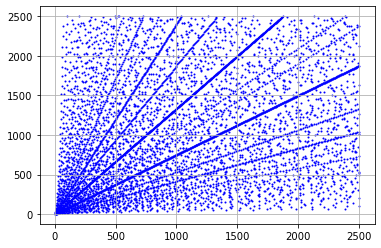
\includegraphics[scale=0.75]{images/2023-03-28-triples_3.png}
\end{figure}

From the lines in the Figure we can clearly see that we can generate non-primitive Pythagorean triples $(kx, ky, kz)$ from a primitive triple $(x,y,z)$. This increases the number of points to $6004$; so we have a density of $\approx 9.6 \cdot 10^{-4}$.

Wikipedia holds some more interesting stuff. The expression

\bee
\frac{1}{2}(z-x)(z-y) = \frac{1}{2}(s^2+t^2 - 2st)(s^2+t^2-(s^2-t^2) = \frac{1}{2} (s-t)^2 2t^2 = t^2(s-t)^2
\eee

is a perfect square. Note that this is only a necessary condition not a sufficient one (i.e. a triple fulfilling the condition need not be a Pythagorean triple).

As an example, for the triple $(6, 12, 18)$, $\frac{1}{2}(z-x)(z-y) = \frac{1}{2} \cdot 12 \cdot 6 = 36$ is a perfect square, but it is not a (primitive) Pythagorean triple: $6^2 + 12^2 \neq 18^2$.

In addition, from above we see that $(z-x) = (s-t)^2$ is a perfect square as is $\frac{1}{2}(z-y) = t^2$. We can check this with the primitive Pythagorean triple $(8, 15, 17)$: $17 - 8 = 9 = 3^2$ and $\frac{1}{2} (17-15) = 1 = 1^2$. Again, this is not a sufficient condition as the example of $(8, 1, 9)$ shows.

In \ref{2023-03-28:entry}, Problem $9$ dealt with Pythagorean triples of the form $(x, y, x+1)$. Also interesting is the case $(x, x+1, z)$. These triples can be constructed by choosing consecutive Pell numbers for $s$ and $t$. Put differently, they are generated by $\frac{s-t}{t}$ being \emph{convergent} tp $\sqrt{2}$ \todo{Explain what convergent is (continued fractions)}.

The first few Pell numbers are $0, 1, 2, 5, 12, \cdots$ and choosing $s = 5, t=2$ we obtain the triple $(20, 21, 29)$.

\subsection{Pell Numbers}

Pell numbers $P_n$ \href{https://oeis.org/A000129}{sequence A000129 in the OEIS} are defined as follows,

\bee
P_n = 2 P_{n-1} + P_{n-2}, \quad P_0 = 0, P_1 = 1
\eee

which is of striking similarity as the Fibonacci numbers. A closed-form expression is given by

\bee
P_n = \frac{(1+\sqrt{2})^n - (1-\sqrt{2})^n}{2 \sqrt{2}}
\eee

The Pell numbers provide approximations for $\sqrt{2}$ as

\bee
\sqrt{2} \approx \frac{P_{n-1} + P_n}{P_n}
\eee

For example, 

\bee
\frac{P_7 + P_8}{P_8} = \frac{169 + 408}{408} \approx 1.414215686 = \sqrt{2} - 2.1239 \cdot 10^{-6}
\eee

which yields a very good approximation.

We can use the Pell numbers to construct Pythagorean triples of the form $(x, x+1, z)$ as shown in the example above for $s = 5, t=2$ which yields the triple $(20, 21, 29)$.

To prove this, we use induction: For the base step, we can use above case $s = 5, t=2$. For the induction step, we construct a triple using $s_1 = P_{n-1}, t_1 = P_{n-2}$. The corresponding $x_1, y_1$ then are

\begin{align*}
    x_1 &= 2P_{n-1} P_{n-2} \\
    y_1 &= P_{n-1}^2 - P_{n-2}^2
\end{align*}

We assume as induction start $y_1, x_1$ differ by one,

\be\label{2023-04-12:eq1}
y_1 - x_1 = P_{n-1}^2 - P_{n-2}^2 - 2 P_{n-1} P_{n-2} = 1
\ee

Now we use the next two Pell numbers $s_2 = P_{n}, t_2 = P_{n-1}$, to obtain the next triple as

\begin{align*}
    x_2 &= 2P_{n} P_{n-1} \\
    y_2 &= P_{n}^2 - P_{n-1}^2
\end{align*}

Therefore the difference, $y_2 - x_2$, becomes,

\bee
    y_2 - x_2 = P_{n}^2 - P_{n-1}^2 - 2P_{n} P_{n-1}
\eee

We want to show that this is equal to $1$, so we somehow need to make use of the induction start \ref{2023-04-12:eq1}. To this end, we use the Pell number definition $P_n = 2 P_{n-1} + P_{n-2}$ and obtain

\begin{align*}
    y_2 - x_2 &= (2 P_{n-1} + P_{n-2})^2 - P_{n-1}^2 - 2(2 P_{n-1} + P_{n-2}) P_{n-1} \\
    &= 4 P_{n-1}^2 + 4 P_{n-1} P_{n-2} + P_{n-2}^2 - P_{n-1}^2 - 4 P_{n-1}^2 - 2 P_{n-1} P_{n-2} \\
    &= 2 P_{n-1} P_{n-2} + P_{n-2}^2 - P_{n-1}^2 \\
    &= - (P_{n-1}^2 - P_{n-2}^2 - 2 P_{n-1} P_{n-2} ) = -1
\end{align*}

This completes the proof; however, note that in the first triple $y_1 > x_1$, whereas $x_2 > y_2$; i.e. the position of the bigger value changes. In our example, we chose $s = 5, t=2$ from which we obtained the triple $(20, 21, 29)$. The next Pell number is then $2 \times 5 + 2 = 12$ and from $s = 12, t = 5$ we obtain the next triple $(120, 119, 169)$. 

\qed

\subsection{Relation to rational Point on the Unit Circle}

See also \cite{Silverman2014}. A point with coordinates $(a,b)$ belongs to the unit circle if $a^2 + b^2 = 1$. A Pythagorean triple is defined by an integer solution to $x^2 + y^2 = z^2$. Dividing this equation by $z^2$, we obtain

\bee
\left( \frac{x}{z} \right)^2 + \left( \frac{y}{z} \right)^2 = 1
\eee

Comparing this with the definition of the unit circle, we see that a tuple $(x,y)$ belonging to a Pythagorean triple, corresponds to a point on the unit circle having rational coordinates.

We are going to use the geometry of the circle $C$ to find all the points on $C$ whose $xy$-coordinates are rational numbers. Notice that the circle has four obvious points with rational coordinates, $(\pm 1, 0)$ and $(0, pm 1)$. Suppose that we take any (rational) number $m$ and look at the line $L$ going through the point $(-1, 0)$ and having slope $m$. The following Figure shows the scenario.

\begin{figure}[H]
    \centering
    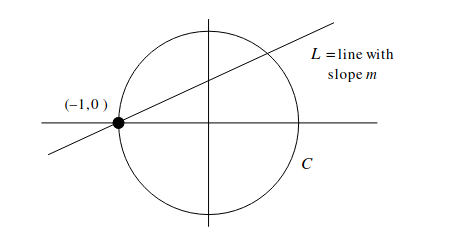
\includegraphics[scale=0.75]{images/2023_04_12_circle_1.png}
\end{figure}

The line $L$ is given by the equation

\bee
y = m(x+1)
\eee

The intersection $C \cap L$ contains two points, one of them being $(-1,0)$. However, we are interested in the other point. This point must fulfill

\bee
x^2 + y^2 = 1, \quad y = m(x+1)
\eee

Inserting the line equation into the circle, we obtain

\bee
x^2 + [m(x+1)]^2 = 1 \rightarrow (m^2+1)x^2 + 2m^2x + (m^2-1) = 0
\eee

We already know that ($-1,0)$ is a solution, to get the other solution, we can therefore divide by $x+1$ and arrive at

\bee
(m^2+1)x + (m^2-1) = 0 \rightarrow x = \frac{1-m^2}{1+m^2}
\eee

Substituting this value of $x$ back into the line equation, we get the solution in rational numbers as

\bee
(x,y) = \left( \frac{1-m^2}{1+m^2}, \frac{2m}{1+m^2} \right)
\eee

So by choosing all rational values for $m$, we get all rational points on the unit circle. To get a connection to the Pythagorean triples, we define $m = u/v$ and obtain

\bee
(x,y) = \left( \frac{u^2-v^2}{u^2+v^2}, \frac{2uv}{u^2+v^2} \right)
\eee

We can clear the denominator and obtain,

\bee
(x,y) = (u^2 - v^2, 2uv) \qed
\eee

\subsection{Misc}

We can generate all primitive Pythagorean triples from two integers, $s, t$ (with conditions on them as $s < t < 0, \gcd(s,t)=1$,

\bee
x = 2st, \quad y = s^2 - t^2, \quad z = s^2 + t^2
\eee

Therefore, there is a one-to-one mapping from the rationals $\frac{m}{n}$ in the interval $[0,1]$ to the primitive Pythagorean triples.

The reverse mapping (from a triple $(x,y,z)$ to the tuple $(s,t)$) is also possible. We consider the two sums $x+z$ and $y+z$: One of them will be twice a square $y + z = 2s^2$, the other, $x + z = 2st + s^2 + t^2 = (s+t)^2$, will be a square, which yields $s+t$.

In order to enumerate primitive Pythagorean triples the rational $\frac{m}{n}$ can be expressed as an ordered pair $(s,t)$ and mapped to an integer using a \emph{pairing function} such as Cantor's pairing function.

\paragraph{Cantor pairing function.} A Cantor pairing function is a bijection

\bee
\pi: \Nc \times \Nc \rightarrow \Nc
\eee

The function is defined by

\bee
\pi(s,t) = \frac{1}{2}(s+t)(s+t+1)+t
\eee

The following Figure shows a plot of the function. It assigns the point $(0,0)$ the value $0$, assigns the "next" point $(0,1)$ the value $1$, then assigns $(1,0)$ the value $2$ and so on. Basically, it numbers the points along the diagonals.

\begin{figure}[H]
    \centering
    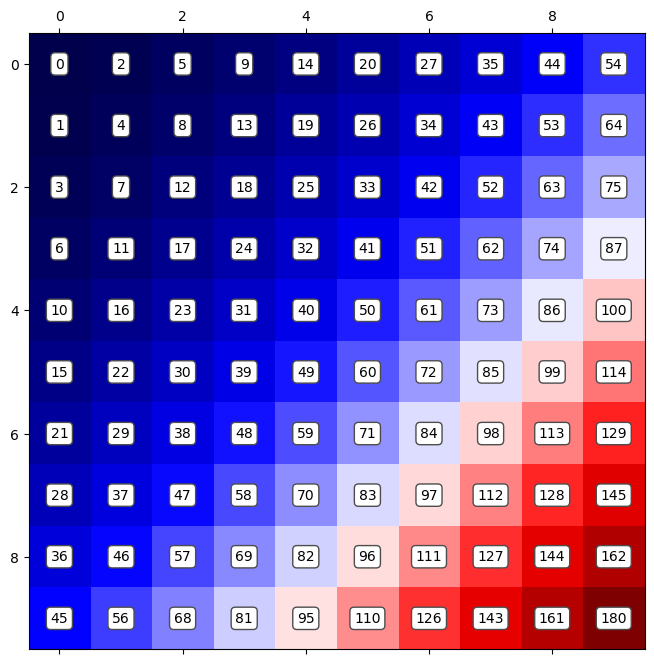
\includegraphics[scale=0.5]{images/2023_04_12_cantor.png}
\end{figure}

Since $\pi(s,t)$ is bijective it is invertible; so knowing $\pi(s,t)$ we can retrieve $s$ and $t$. The calculation is a bit tricky; see eg \href{https://en.m.wikipedia.org/wiki/Pairing_function}{Wikipedia}.


If we chose our pairing function for the primitive Pythagorean triples to be $\pi(s,t)$, then we get for example,

\bee
s = 5, t = 2 \rightarrow(5,2) = 30
\eee

and this corresponds to the primitive Pythagorean triple $(20,21,29)$. The corresponding OEIS sequence is \href{https://oeis.org/A277557}{A277557}.


\paragraph{Trees of Pythagorean triples.} There is a result that \emph{all} primitive Pythagorean triples can be generated from the triple $(3,4,5)$ by applying linear transformations. More precisely, three linear transforms are applied to one triple, yielding $3$ different primitive Pythagorean triples. This procedure does not create any duplicates, so the whole process generates a tree of Pythagorean triples with $(3,4,5)$ as root node.

The three transformations are denoted as $T_1, T_2, T_3$; each transformation takes a triple $(x,y,z)$ as input and yields a triple $(x', y', z')$. The transformations are given by the following equations (cf \href{https://en.m.wikipedia.org/wiki/Pythagorean_triple}{here})

\begin{align}
    T_1&: x' = x - 2y + 2z, y' = 2x-y+2z, z' = 2x-2y+3z \\
    T_2&: x' = x + 2y + 2z, y' = 2x+y+2z, z' = 2x + 2y + 3z \\
    T_3&: x' = -x+2y+2z, y' = -2x+y+2z, z' = -2x + 2y + 3z
\end{align}

Starting from $(3,4,5)$, the first transformation yields the triple $(5, 12, 13)$, the second yields $(21, 20, 29)$ and finlly the third yields $(15, 8, 17)$.


%%% Local Variables:
%%% mode: latex
%%% TeX-master: "journal"
%%% End:
